\documentclass[12pt, letterpaper]{article}
\usepackage[titletoc,title]{appendix}
\usepackage{color}
\usepackage{booktabs}
\usepackage[tableposition=top]{caption}
\newcommand\fnote[1]{\captionsetup{font=small}\caption*{#1}}

\usepackage[usenames,dvipsnames,svgnames,table]{xcolor}
\definecolor{dark-red}{rgb}{0.75,0.10,0.10} 
\usepackage[margin=1in]{geometry}
\usepackage[linkcolor=dark-red,
            colorlinks=true,
            urlcolor=blue,
            pdfstartview={XYZ null null 1.00},
            pdfpagemode=UseNone,
            citecolor={dark-red},
            pdftitle={SI for Pwned}]{hyperref}
%\usepackage{multibib}
\usepackage{geometry} % see geometry.pdf on how to lay out the page. There's lots.
\geometry{letterpaper}               % This is 8.5x11 paper. Options are a4paper or a5paper or other... 
\usepackage{graphicx}                % Handles inclusion of major graphics formats and allows use of 
\usepackage{amsfonts,amssymb,amsbsy}
\usepackage{amsxtra}
\usepackage{natbib}
\DeclareRobustCommand{\firstsecond}[2]{#1}
\usepackage{verbatim}
\setcitestyle{round,semicolon,aysep={},yysep={;}}
\usepackage{setspace}             % Permits line spacing control. Options are \doublespacing, \onehalfspace
\usepackage{sectsty}             % Permits control of section header styles
\usepackage{lscape}
\usepackage{fancyhdr}             % Permits header customization. See header section below.
\usepackage{url}                 % Correctly formats URLs with the \url{} tag
\usepackage{fullpage}             %1-inch margins
\usepackage{multirow}
\usepackage{rotating}
\setlength{\parindent}{3em}
\usepackage{subcaption}
\usepackage{float}

%\usepackage[T1]{fontenc}
%\usepackage{bm}
\usepackage{lmodern}
%\usepackage{libertine}
%\usepackage{gfsdidot}
\usepackage{chngcntr}

\title{\Large{Supporting Information for Pwned:  The Risk of Exposure From Data Breaches}\footnote{Data and scripts behind the analysis presented here can be downloaded from \url{http://github.com/themains/pwned}.
}}

\author{Gaurav Sood\thanks{Gaurav can be reached at \href{mailto:gsood07@gmail.com}{\footnotesize{\texttt{gsood07@gmail.com}}}} \and Ken Cor\thanks{Ken can be reached at: \href{mailto:mcor@ualberta.ca}{\footnotesize{\texttt{mcor@ualberta.ca}}}}\vspace{.5cm}}

\begin{document}
\maketitle

\begin{center}
%\vspace{.5cm}\textbf{NB:} Preliminary draft. Please do not cite without permission.\vspace{1.5cm}
\end{center}

\begin{comment}

setwd(paste0(githubdir, "pwned_dev/ms/"))
tools::texi2dvi("pwned_si.tex", pdf = TRUE, clean = TRUE)
setwd(githubdir)

\end{comment}

\renewcommand{\thesection}{SI \arabic{section}}
\renewcommand\thetable{\thesection.\arabic{table}}  
\renewcommand\thefigure{\thesection.\arabic{figure}}
\counterwithin{figure}{section}

\clearpage
\section{Tables}
\label{fig:si_tables}

The missing entries reflect cases where we do not have commensurate categories in our data. The largest differences we see are on race and ethnicity, a variable where our coding differs from CPS in meaningful ways. 

% latex table generated in R 3.5.3 by xtable 1.8-4 package
% Mon Apr 29 20:09:37 2019
\begin{table}[!htb]
\centering
\caption{Comparison Between YouGov and CPS 2018} 
\label{table:cps_yg}
\begingroup\small
\begin{tabular}{lrrr}
  \hline
 & cps & yg & diff \\ 
  \hline
Age &  &  &  \\ 
  18 to 25 & 0.14 & 0.13 & 0.01 \\ 
  26 to 35 & 0.18 & 0.18 & 0.00 \\ 
  36 to 50 & 0.25 & 0.23 & 0.02 \\ 
  51 to 65 & 0.25 & 0.26 & -0.01 \\ 
  66 to 80+ & 0.19 & 0.18 & 0.01 \\ 
  Sex &  &  &  \\ 
  Male & 0.48 & 0.51 & -0.03 \\ 
  Female & 0.52 & 0.49 & 0.03 \\ 
  Race &  &  &  \\ 
  White alone & 0.78 & 0.64 & 0.14 \\ 
  Black or African American alone & 0.13 & 0.12 & 0.01 \\ 
  American Indian and Alaska Native alone & 0.01 & 0.01 & 0.00 \\ 
  Asian alone & 0.06 &  &  \\ 
  Native Hawaiian and Other Pacific Islander alone & 0.00 &  &  \\ 
  Two or more races & 0.02 &  &  \\ 
  Educational Attainment &  &  &  \\ 
  No high school diploma & 0.11 & 0.07 & 0.04 \\ 
  High school or equivalent & 0.29 & 0.33 & -0.04 \\ 
  Some college, less than 4-yr degree & 0.28 & 0.31 & -0.03 \\ 
  Bachelor's degree or higher & 0.32 & 0.29 & 0.03 \\ 
   \hline
\end{tabular}
\endgroup
\end{table}

\clearpage


% Table created by stargazer v.5.2.2 by Marek Hlavac, Harvard University. E-mail: hlavac at fas.harvard.edu
% Date and time: Sat, Apr 27, 2019 - 5:55:59 PM
\begin{table}[!htbp] \centering 
  \caption{Number of Breaches by Race/Ethnicity} 
  \label{tab:race_breaches} 
\begin{tabular}{@{\extracolsep{5pt}}lc} 
\\[-1.8ex]\hline 
\hline \\[-1.8ex] 
 & \multicolumn{1}{c}{\textit{Dependent variable:}} \\ 
\cline{2-2} 
\\[-1.8ex] & Number of Breaches \\ 
\hline \\[-1.8ex] 
 Black & .04 \\ 
  & (.12) \\ 
  Hispanic/Latino & $-$.62$^{***}$ \\ 
  & (.10) \\ 
  Asian & $-$.30 \\ 
  & (.23) \\ 
  Native American & $-$.16 \\ 
  & (.36) \\ 
  Middle Eastern & $-$.46$^{**}$ \\ 
  & (.24) \\ 
  Mixed Race & $-$.67$^{**}$ \\ 
  & (.29) \\ 
  Other & $-$.20 \\ 
  & (.73) \\ 
  Constant & 3.12$^{***}$ \\ 
  & (.05) \\ 
 \hline \\[-1.8ex] 
Observations & 5,000 \\ 
R$^{2}$ & .01 \\ 
Adjusted R$^{2}$ & .01 \\ 
\hline 
\hline \\[-1.8ex] 
\textit{Note:}  & \multicolumn{1}{r}{$^{*}$p$<$0.1; $^{**}$p$<$0.05; $^{***}$p$<$0.01} \\ 
\end{tabular} 
\end{table} 

\clearpage


% Table created by stargazer v.5.2.2 by Marek Hlavac, Harvard University. E-mail: hlavac at fas.harvard.edu
% Date and time: Sun, Feb 17, 2019 - 2:48:10 PM
\begin{table}[!htbp] \centering 
  \caption{Number of Breaches by Sex} 
  \label{} 
\begin{tabular}{@{\extracolsep{5pt}}lc} 
\\[-1.8ex]\hline 
\hline \\[-1.8ex] 
 & \multicolumn{1}{c}{\textit{Dependent variable:}} \\ 
\cline{2-2} 
\\[-1.8ex] & Number of Breaches \\ 
\hline \\[-1.8ex] 
 Male & $-$.35$^{***}$ \\ 
  & (.07) \\ 
  Constant & 3.17$^{***}$ \\ 
  & (.05) \\ 
 \hline \\[-1.8ex] 
Observations & 5,000 \\ 
R$^{2}$ & .004 \\ 
Adjusted R$^{2}$ & .004 \\ 
\hline 
\hline \\[-1.8ex] 
\textit{Note:}  & \multicolumn{1}{r}{$^{*}$p$<$0.1; $^{**}$p$<$0.05; $^{***}$p$<$0.01} \\ 
\end{tabular} 
\end{table} 

\clearpage


% Table created by stargazer v.5.2.2 by Marek Hlavac, Harvard University. E-mail: hlavac at fas.harvard.edu
% Date and time: Sat, Apr 27, 2019 - 5:55:59 PM
\begin{table}[!htbp] \centering 
  \caption{Number of Breaches by Education} 
  \label{tab:educ_breaches} 
\begin{tabular}{@{\extracolsep{5pt}}lc} 
\\[-1.8ex]\hline 
\hline \\[-1.8ex] 
 & \multicolumn{1}{c}{\textit{Dependent variable:}} \\ 
\cline{2-2} 
\\[-1.8ex] & Number of Breaches \\ 
\hline \\[-1.8ex] 
 HS Grad. & .54$^{***}$ \\ 
  & (.16) \\ 
  Some College & .69$^{***}$ \\ 
  & (.16) \\ 
  2-year College Degree & .72$^{***}$ \\ 
  & (.18) \\ 
  4-year College Degree & .87$^{***}$ \\ 
  & (.17) \\ 
  Postgrad Degree & .85$^{***}$ \\ 
  & (.18) \\ 
  Constant & 2.35$^{***}$ \\ 
  & (.14) \\ 
 \hline \\[-1.8ex] 
Observations & 5,000 \\ 
R$^{2}$ & .01 \\ 
Adjusted R$^{2}$ & .01 \\ 
\hline 
\hline \\[-1.8ex] 
\textit{Note:}  & \multicolumn{1}{r}{$^{*}$p$<$0.1; $^{**}$p$<$0.05; $^{***}$p$<$0.01} \\ 
\end{tabular} 
\end{table} 


\clearpage

% Table created by stargazer v.5.2.2 by Marek Hlavac, Harvard University. E-mail: hlavac at fas.harvard.edu
% Date and time: Mon, Feb 11, 2019 - 7:51:27 PM
\begin{table}[!htbp] \centering 
  \caption{Number of Breaches by Age} 
  \label{} 
\begin{tabular}{@{\extracolsep{5pt}}lc} 
\\[-1.8ex]\hline 
\hline \\[-1.8ex] 
 & \multicolumn{1}{c}{\textit{Dependent variable:}} \\ 
\cline{2-2} 
\\[-1.8ex] & Number of Breaches \\ 
\hline \\[-1.8ex] 
 ns(age, 2)1 & 2.23$^{***}$ \\ 
  & (.20) \\ 
  ns(age, 2)2 & $-$.90$^{***}$ \\ 
  & (.21) \\ 
  Constant & 2.01$^{***}$ \\ 
  & (.09) \\ 
 \hline \\[-1.8ex] 
Observations & 5,000 \\ 
R$^{2}$ & .03 \\ 
Adjusted R$^{2}$ & .03 \\ 
\hline 
\hline \\[-1.8ex] 
\textit{Note:}  & \multicolumn{1}{r}{$^{*}$p$<$0.1; $^{**}$p$<$0.05; $^{***}$p$<$0.01} \\ 
\end{tabular} 
\end{table} 


\clearpage
\section{Figures}
\label{fig:si_figs}

\begin{figure}[H]
  \centering
  \captionsetup{font={small,it}}
   \caption{Relationship Between Race and Number of Breaches
  \label{fig:race_breaches}}
    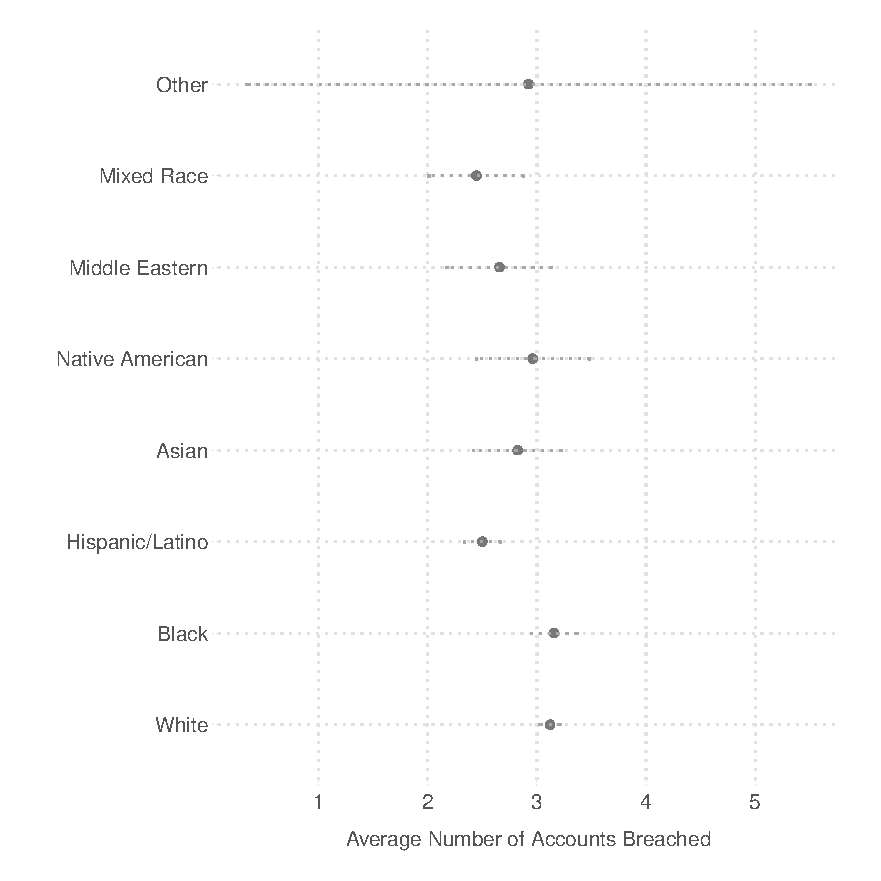
\includegraphics[scale=.75]{../figs/race_pwned.pdf}
\end{figure}
\clearpage

\begin{figure}[H]
  \centering
  \captionsetup{font={small,it}}
   \caption{Relationship Between Sex and Number of Breaches  
  \label{fig:sex_breaches}}
    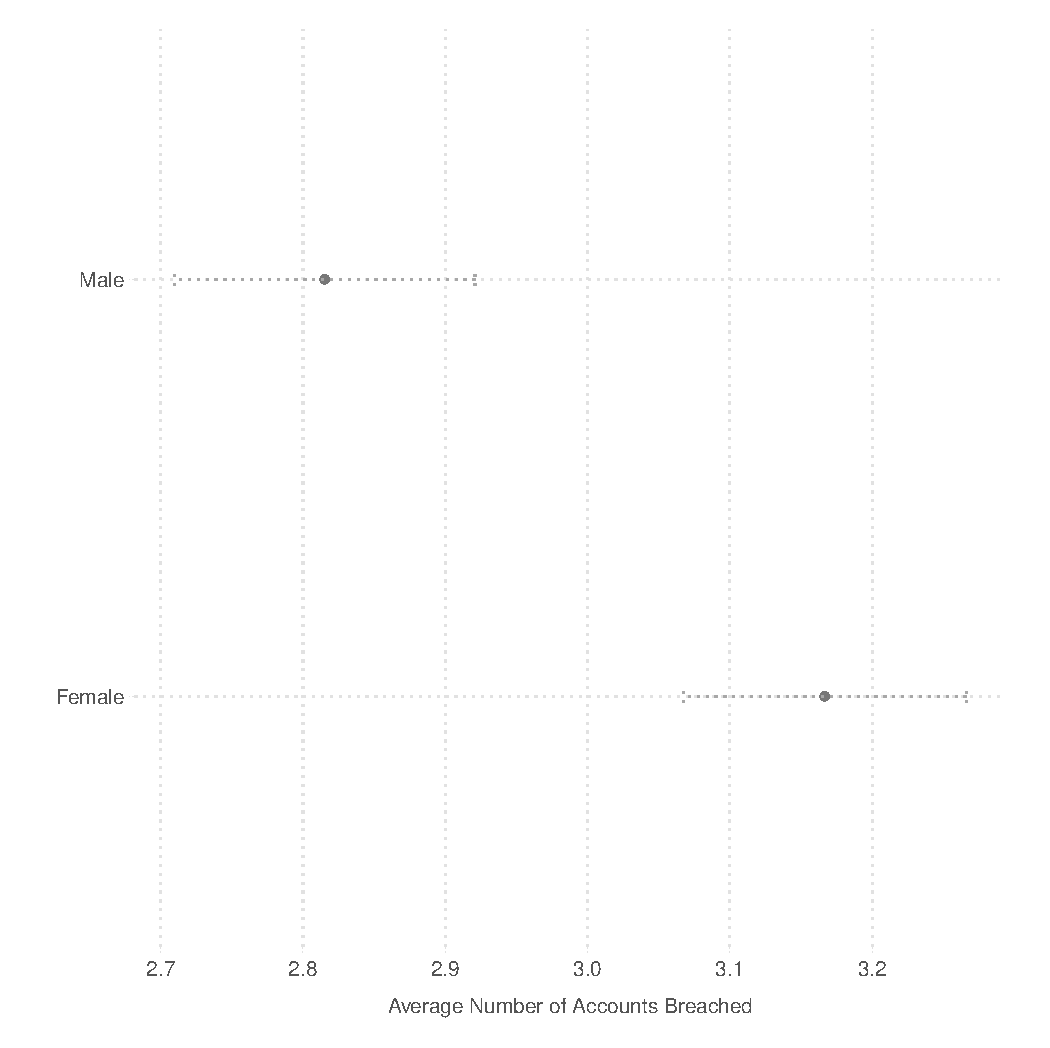
\includegraphics[scale=.75]{../figs/sex_pwned.pdf}
\end{figure}
\clearpage

\begin{figure}[H]
  \centering
  \captionsetup{font={small,it}}
   \caption{Relationship Between Education and Number of Breaches 
  \label{fig:educ_breaches}}
    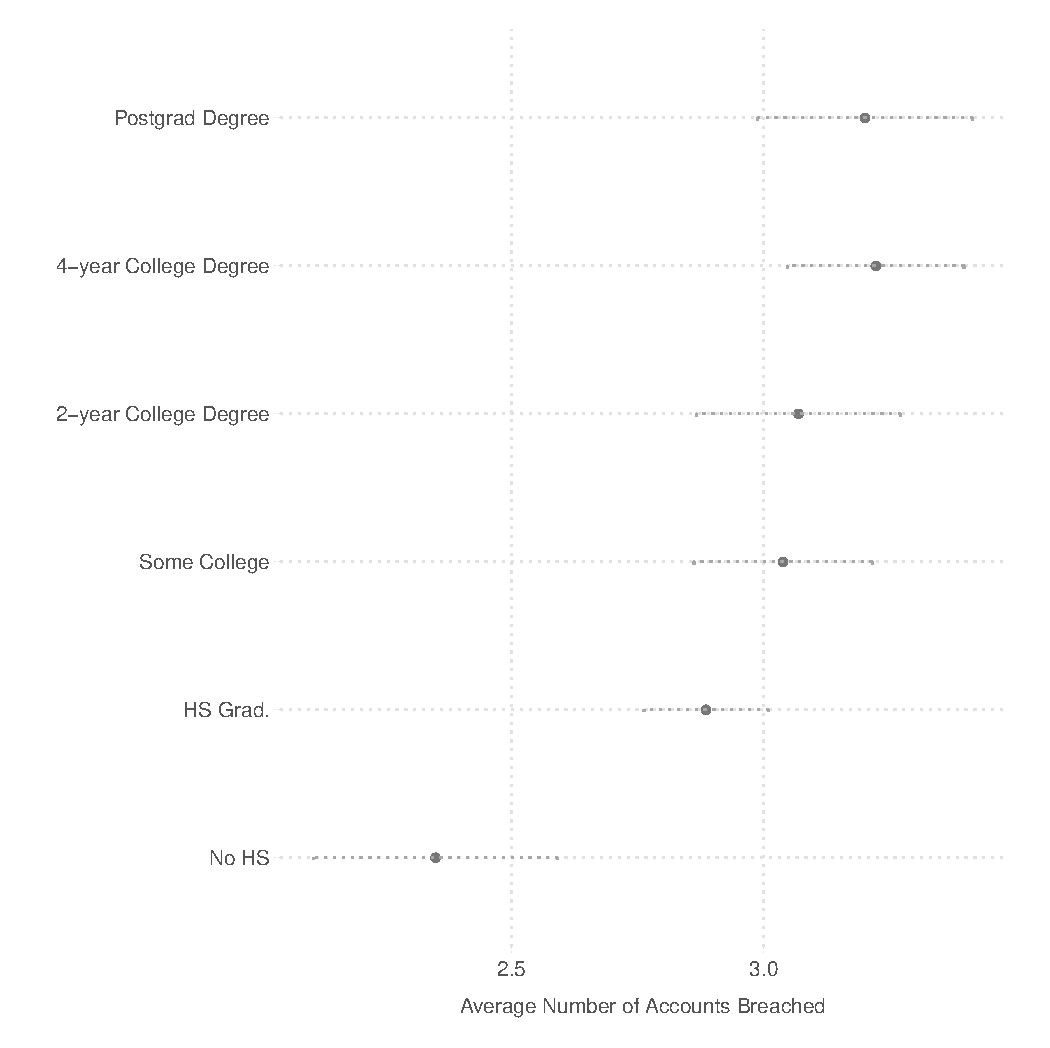
\includegraphics[scale=.75]{../figs/educ_pwned.pdf}
\end{figure}
\clearpage

\begin{figure}[H]
  \centering
  \captionsetup{font={small,it}}
   \caption{Relationship Between Age and Number of Breaches  
  \label{fig:age_breaches}}
    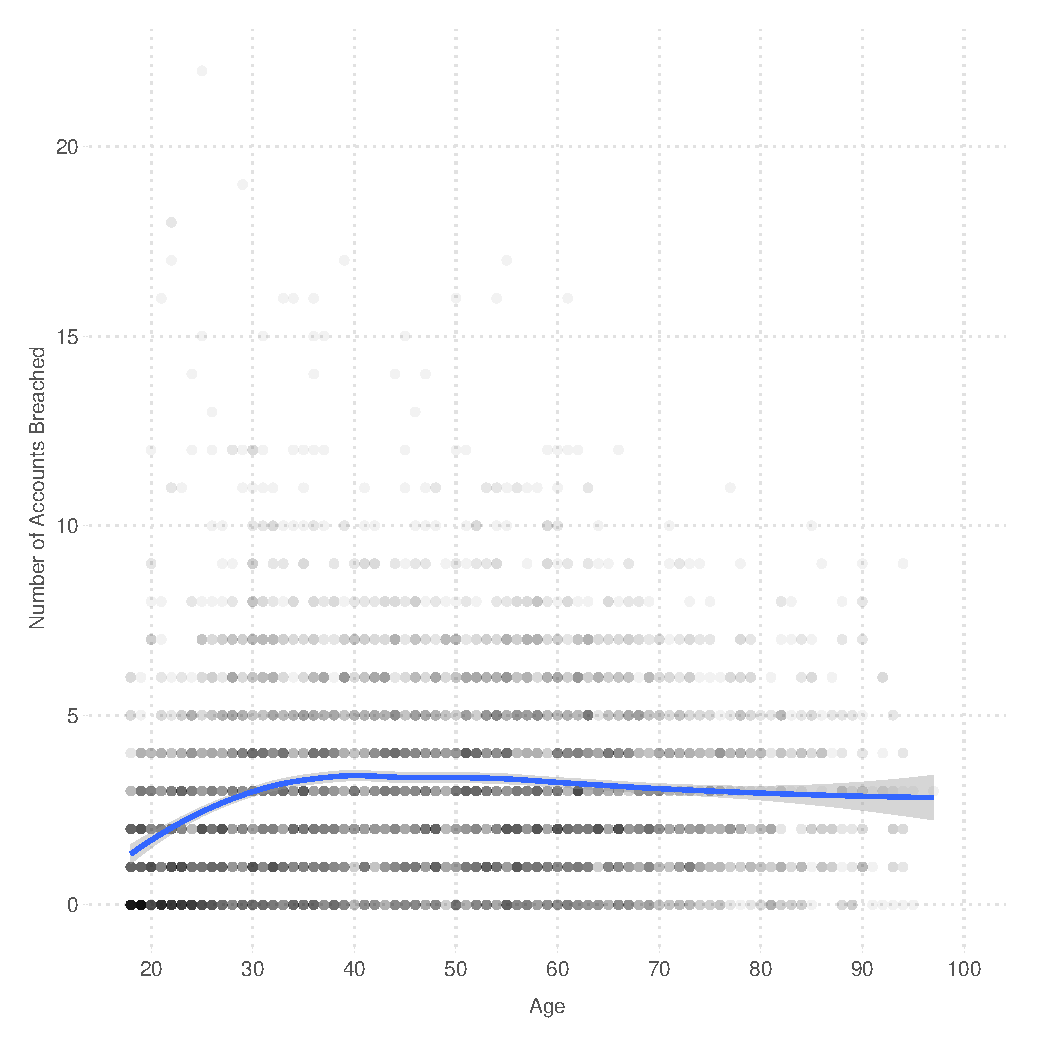
\includegraphics[scale=.75]{../figs/age_pwned.pdf}
\end{figure}

\end{document}